\hypertarget{lists-and-arrays}{%
\chapter{Lists and Arrays}\label{lists-and-arrays}}

In the previous chapter we used tuples to represent latitude and
longitude. In this chapter, you'll see how to use tuples more generally
to represent a sequence of values. And we'll see two more ways to
represent sequences: lists and arrays.

You might wonder why we need three ways to represent the same thing.
Most of the time you don't, but each of them has different capabilities.
For work with data, we will use arrays most of the time.

As an example, we will use a small dataset from an article in \emph{The
Economist} about the price of sandwiches. It's a silly example, but I'll
use it to introduce the idea of relative differences and different ways
to summarize them.

\hypertarget{tuples}{%
\section{Tuples}\label{tuples}}

A tuple is a sequence of elements. When we use a tuple to represent
latitude and longitude, the sequence only contains two elements, and
they are both floating-point numbers. But in general a tuple can contain
any number of elements, and the elements can be values of any type. The
following is a tuple of three integers:

\begin{lstlisting}[]
1, 2, 3
(@\dashfill@)
@@@(1, 2, 3)@@@
\end{lstlisting}

Notice that when Python displays a tuple, it puts the elements in
parentheses. When you type a tuple, you can put it in parentheses if you
think it is easier to read that way, but you don't have to.

The elements can be any type. Here's a tuple of strings:

\begin{lstlisting}[]
'Data', 'Science'
(@\dashfill@)
@@@('Data', 'Science')@@@
\end{lstlisting}

The elements don't have to be the same type. Here's a tuple with a
string, an integer, and a floating-point number.

\begin{lstlisting}[]
'one', 2, 3.14159 
(@\dashfill@)
@@@('one', 2, 3.14159)@@@
\end{lstlisting}

If you have a string, you can convert it to a tuple using the
\passthrough{\lstinline!tuple!} function:

\begin{lstlisting}[]
tuple('DataScience')
(@\dashfill@)
@@@('D', 'a', 't', 'a', 'S', 'c', 'i', 'e', 'n', 'c', 'e')@@@
\end{lstlisting}

The result is a tuple of single-character strings.

When you create a tuple, the parentheses are optional, but the commas
are required. So how do you think you create a tuple with a single
element? You might be tempted to write:

\begin{lstlisting}[]
x = (5)
x
(@\dashfill@)
@@@5@@@
\end{lstlisting}

But you will find that the result is just a number, not a tuple. To make
a tuple with a single element, you need a comma:

\begin{lstlisting}[]
t = 5,
t
(@\dashfill@)
@@@(5,)@@@
\end{lstlisting}

That might look funny, but it does the job.

\hypertarget{lists}{%
\section{Lists}\label{lists}}

Python provides another way to store a sequence of elements: a list.

To create a list, you put a sequence of elements in square brackets.

\begin{lstlisting}[]
[1, 2, 3]
(@\dashfill@)
@@@[1, 2, 3]@@@
\end{lstlisting}

Lists and tuples are very similar. They can contain any number of
elements, the elements can be any type, and the elements don't have to
be the same type. The difference is that you can modify a list; tuples
are immutable (cannot be modified). This difference will matter later,
but for now we can ignore it.

When you make a list, the brackets are required, but if there is a
single element, you don't need a comma. So you can make a list like
this:

\begin{lstlisting}[]
single = [5]
\end{lstlisting}

It is also possible to make a list with no elements, like this:

\begin{lstlisting}[]
empty = []
\end{lstlisting}

The \passthrough{\lstinline!len!} function returns the length (number of
elements) in a list or tuple.

\begin{lstlisting}[]
len([1, 2, 3]), len(single), len(empty)
(@\dashfill@)
@@@(3, 1, 0)@@@
\end{lstlisting}

\textbf{Exercise:} Create a list with 4 elements; then use
\passthrough{\lstinline!type!} to confirm that it's a list, and
\passthrough{\lstinline!len!} to confirm that it has 4 elements.

There's a lot more we could do with lists, but that's enough to get
started. In the next section, we'll use lists to store data about
sandwich prices.

\hypertarget{sandwiches}{%
\section{Sandwiches}\label{sandwiches}}

In September 2019, \emph{The Economist} published an article comparing
sandwich prices in Boston and London:
``\href{https://www.economist.com/finance-and-economics/2019/09/07/why-americans-pay-more-for-lunch-than-britons-do}{Why
Americans pay more for lunch than Britons do}''. It includes this graph
showing prices of several sandwiches in the two cities:

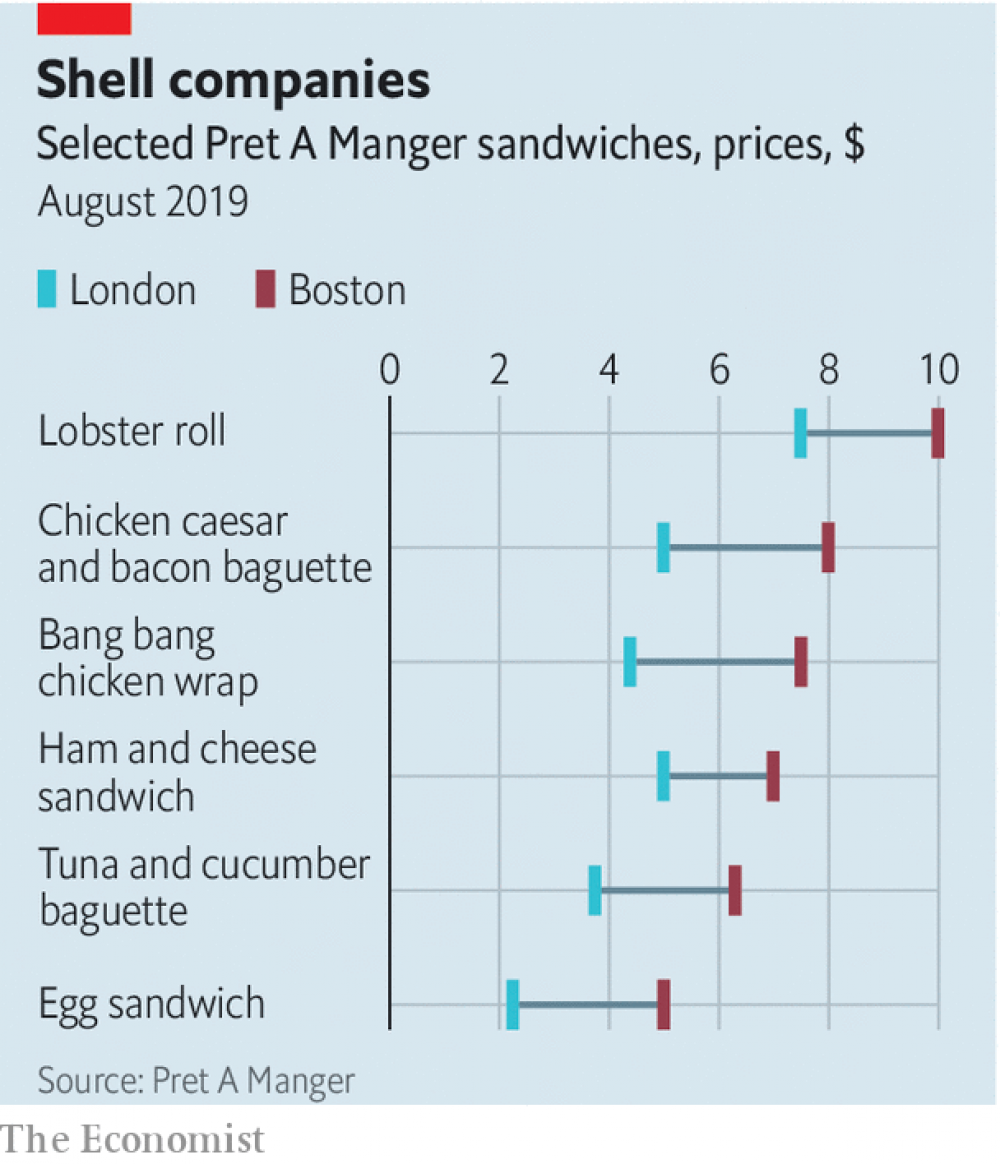
\includegraphics{figs/20190907_FNC941.png}

Here are the sandwich names from the graph, as a list of strings.

\begin{lstlisting}[]
name_list = [
    'Lobster roll',
    'Chicken caesar',
    'Bang bang chicken',
    'Ham and cheese',
    'Tuna and cucumber',
    'Egg'
]
\end{lstlisting}

I contacted \emph{The Economist} to ask for the data they used to create
that graph, and they were kind enough to share it with me. Here are the
sandwich prices in Boston:

\begin{lstlisting}[]
boston_price_list = [9.99, 7.99, 7.49, 7.00, 6.29, 4.99]
\end{lstlisting}

Here are the prices in London, converted to dollars at \$1.25 / £1.

\begin{lstlisting}[]
london_price_list = [7.5, 5, 4.4, 5, 3.75, 2.25]
\end{lstlisting}

Lists provide some arithmetic operators, but they might not do what you
want. For example, you can ``add'' two lists:

\begin{lstlisting}[]
boston_price_list + london_price_list
(@\dashfill@)
@@@[9.99, 7.99, 7.49, 7.0, 6.29, 4.99, 7.5, 5, 4.4, 5, 3.75, 2.25]@@@
\end{lstlisting}

But it concatenates the two lists, which is not very useful in this
example. To compute differences between prices, you might try
subtracting lists, but you would get an error.\\
We can solve this problem with a NumPy array.

\hypertarget{numpy-arrays}{%
\section{NumPy Arrays}\label{numpy-arrays}}

We've already seen that the NumPy library provides math functions. It
also provides a type of sequence called an array. You can create a new
array with the \passthrough{\lstinline!np.array!} function, starting
with a list or tuple.

\begin{lstlisting}[]
import numpy as np

boston_price_array = np.array(boston_price_list)
london_price_array = np.array(london_price_list)
\end{lstlisting}

The type of the result is \passthrough{\lstinline!numpy.ndarray!}.

\begin{lstlisting}[]
type(boston_price_array)
(@\dashfill@)
@@@numpy.ndarray@@@
\end{lstlisting}

The ``nd'' stands for ``n-dimensional'', which indicates that NumPy
arrays can have any number of dimensions. But for now we will work with
one-dimensional sequences. If you display an array, Python displays the
elements:

\begin{lstlisting}[]
boston_price_array
(@\dashfill@)
@@@array([9.99, 7.99, 7.49, 7.  , 6.29, 4.99])@@@
\end{lstlisting}

You can also display the ``data type'' of the array, which is the type
of the elements:

\begin{lstlisting}[]
boston_price_array.dtype
(@\dashfill@)
@@@dtype('float64')@@@
\end{lstlisting}

\passthrough{\lstinline!float64!} means that the elements are
floating-point numbers that take up 64 bits each. You don't need to know
about the storage format of these numbers, but if you are curious, you
can read about it at
\url{https://en.wikipedia.org/wiki/Floating-point_arithmetic\#Internal_representation}.

The elements of a NumPy array can be any type, but they all have to be
the same type. Most often the elements are numbers, but you can also
make an array of strings.

\begin{lstlisting}[]
name_array = np.array(name_list)
name_array
(@\dashfill@)
@@@array(['Lobster roll', 'Chicken caesar', 'Bang bang chicken',
       'Ham and cheese', 'Tuna and cucumber', 'Egg'], dtype='<U17')@@@
\end{lstlisting}

In this example, the \passthrough{\lstinline!dtype!} is
\passthrough{\lstinline!<U17!}. The \passthrough{\lstinline!U!}
indicates that the elements are Unicode strings; Unicode is the standard
Python uses to represent strings.

Now, here's why NumPy arrays are useful: they can do arithmetic. For
example, to compute the differences between Boston and London prices, we
can write:

\begin{lstlisting}[]
differences = boston_price_array - london_price_array
differences
(@\dashfill@)
@@@array([2.49, 2.99, 3.09, 2.  , 2.54, 2.74])@@@
\end{lstlisting}

Subtraction is done ``elementwise''; that is, NumPy lines up the two
arrays and subtracts corresponding elements. The result is a new array.

\hypertarget{mean-and-standard-deviation}{%
\section{Mean and standard
deviation}\label{mean-and-standard-deviation}}

NumPy provides functions that compute statistical summaries like the
mean:

\begin{lstlisting}[]
np.mean(differences)
(@\dashfill@)
@@@2.6416666666666666@@@
\end{lstlisting}

So we could describe the difference in prices like this: ``Sandwiches in
Boston are more expensive by \$2.64, on average''. We could also compute
the means first, and then compute their difference:

\begin{lstlisting}[]
np.mean(boston_price_array) - np.mean(london_price_array)
(@\dashfill@)
@@@2.6416666666666675@@@
\end{lstlisting}

And that turns out to be the same thing: the difference in means is the
same as the mean of the differences. As an aside, many of the NumPy
functions also work with lists, so we could also do this:

\begin{lstlisting}[]
np.mean(boston_price_list) - np.mean(london_price_list)
(@\dashfill@)
@@@2.6416666666666675@@@
\end{lstlisting}

\textbf{Exercise:} Standard deviation is way to quantify the variability
in a set of numbers. The NumPy function that computes standard deviation
is \passthrough{\lstinline!np.std!}.

Compute the standard deviation of sandwich prices in Boston and London.
By this measure, which set of prices is more variable?

\textbf{Exercise:} The definition of the mean, in math notation, is

\(\mu = \frac{1}{N} \sum_i x_i\)

where \(x\) is a sequence of elements, \(x_i\) is the element with index
\(i\), and \(N\) is the number of elements. The definition of standard
deviation is

\(\sigma = \sqrt{\frac{1}{N} \sum_i (x_i - \mu)^2}\)

Compute the standard deviation of
\passthrough{\lstinline!boston\_price\_list!} using NumPy functions
\passthrough{\lstinline!np.mean!} and \passthrough{\lstinline!np.sqrt!}
and see if you get the same result as \passthrough{\lstinline!np.std!}.

Note: You can (and should) do this exercise using only features we have
discussed so far.

Note: This definition of standard deviation is sometimes called the
``population standard deviation''. You might have seen another
definition with \(N-1\) in the denominator; that's the ``sample standard
deviation''. We'll use the population standard deviation for now and
come back to this issue later.

\hypertarget{relative-difference}{%
\section{Relative Difference}\label{relative-difference}}

In the previous section we computed differences between prices. But
often when we make this kind of comparison, we are interested in
\textbf{relative difference}, which are differences expressed as a
fraction or percentage of a quantity.

Taking the lobster roll as an example, the difference in price is:

\begin{lstlisting}[]
9.99 - 7.5
(@\dashfill@)
@@@2.49@@@
\end{lstlisting}

We can express that difference as a fraction of the London price, like
this:

\begin{lstlisting}[]
(9.99 - 7.5) / 7.5
(@\dashfill@)
@@@0.332@@@
\end{lstlisting}

Or as a \emph{percentage} of the London price, like this:

\begin{lstlisting}[]
(9.99 - 7.5) / 7.5 * 100
(@\dashfill@)
@@@33.2@@@
\end{lstlisting}

So we might say that the lobster roll is 33\% more expensive in Boston.
But putting London in the denominator was an arbitrary choice. We could
also compute the difference as a percentage of the Boston price:

\begin{lstlisting}[]
(9.99 - 7.5) / 9.99 * 100
(@\dashfill@)
@@@24.924924924924927@@@
\end{lstlisting}

If we do that calculation, we might say the lobster roll is 25\% cheaper
in London. When you read this kind of comparison, you should make sure
you understand which quantity is in the denominator, and you might want
to think about why that choice was made. In this example, if you want to
make the difference seem bigger, you might put London prices in the
denominator.

If we do the same calculation with the arrays
\passthrough{\lstinline!boston\_price\_array!} and
\passthrough{\lstinline!boston\_price\_array!}, we can compute the
relative differences for all sandwiches:

\begin{lstlisting}[]
differences = boston_price_array - london_price_array
relative_differences = differences / london_price_array
relative_differences
(@\dashfill@)
@@@array([0.332     , 0.598     , 0.70227273, 0.4       , 0.67733333,
       1.21777778])@@@
\end{lstlisting}

And the percent differences.

\begin{lstlisting}[]
percent_differences = relative_differences * 100
percent_differences
(@\dashfill@)
@@@array([ 33.2       ,  59.8       ,  70.22727273,  40.        ,
        67.73333333, 121.77777778])@@@
\end{lstlisting}

\hypertarget{summarizing-relative-differences}{%
\section{Summarizing Relative
Differences}\label{summarizing-relative-differences}}

Now let's think about how to summarize an array of percentage
differences. One option is to report the range, which we can compute
with \passthrough{\lstinline!np.min!} and
\passthrough{\lstinline!np.max!}.

\begin{lstlisting}[]
np.min(percent_differences), np.max(percent_differences)
(@\dashfill@)
@@@(33.2, 121.77777777777779)@@@
\end{lstlisting}

The lobster roll is only 33\% more expensive in Boston; the egg sandwich
is 121\% percent more (that is, more than twice the price).

\textbf{Exercise:} What are the percent differences if we put the Boston
prices in the denominator? What is the range of those differences? Write
a sentence that summarizes the results.

Another way to summarize percentage differences is to report the mean.

\begin{lstlisting}[]
np.mean(percent_differences)
(@\dashfill@)
@@@65.4563973063973@@@
\end{lstlisting}

So we might say, on average, sandwiches are 65\% more expensive in
Boston. But another way to summarize the data is to compute the mean
price in each city, and then compute the percentage difference of the
means:

\begin{lstlisting}[]
boston_mean = np.mean(boston_price_array)
london_mean = np.mean(london_price_array)

(boston_mean - london_mean) / london_mean * 100
(@\dashfill@)
@@@56.81003584229393@@@
\end{lstlisting}

So we might say that the average sandwich price is 56\% higher in
Boston. As this example demonstrates:

\begin{itemize}
\item
  With relative and percentage differences, the mean of the differences
  is not the same as the difference of the means.
\item
  When you report data like this, you should think about different ways
  to summarize the data.
\item
  When you read a summary of data like this, make sure you understand
  what summary was chosen and what it means.
\end{itemize}

In this example, I think the second option (the relative difference in
the means) is more meaningful, because it reflects the difference in
price between ``baskets of goods'' that include one of each sandwich.

\hypertarget{debugging}{%
\section{Debugging}\label{debugging}}

So far, most of the exercises have only required a few lines of code. If
you made errors along the way, you probably found them quickly.

As we go along, the exercises will be more substantial, and you may find
yourself spending more time debugging. Here are a couple of suggestions
to help you find errors quickly -- and avoid them in the first place.

\begin{itemize}
\item
  Most importantly, you should develop code incrementally; that is, you
  should write a small amount of code and test it. If it works, add more
  code; otherwise, debug what you have.
\item
  Conversely, if you have written too much code, and you are having a
  hard time debugging it, split it into smaller chunks and debug them
  separately.
\end{itemize}

For example, suppose you want to compute, for each sandwich in the
sandwich list, the midpoint of the Boston and London prices. As a first
draft, you might write something like this:

\begin{lstlisting}[]
boston_price_list = [9.99, 7.99, 7.49, 7, 6.29, 4.99]
london_price_list = [7.5, 5, 4.4, 5, 3.75, 2.25]

midpoint_price = np.mean(boston_price_list + london_price_list)
midpoint_price
(@\dashfill@)
@@@5.970833333333334@@@
\end{lstlisting}

This code runs, and it produces an answer, but the answer is a single
number rather than the list we were expecting.

You might have already spotted the error, but let's suppose you did not.
To debug this code, I would start by splitting the computation into
smaller steps and displaying the intermediate results. For example, we
might add the two lists and display the result, like this.

\begin{lstlisting}[]
total_price = boston_price_list + london_price_list
total_price
(@\dashfill@)
@@@[9.99, 7.99, 7.49, 7, 6.29, 4.99, 7.5, 5, 4.4, 5, 3.75, 2.25]@@@
\end{lstlisting}

Looking at the result, we see that it did not add the sandwich prices
elementwise, as we intended. Because the arguments are lists, the
\passthrough{\lstinline!+!} operator concatenates them rather than
adding the elements.

We can solve this problem by converting the lists to arrays.

\begin{lstlisting}[]
boston_price_array = np.array(boston_price_list)
london_price_array = np.array(london_price_list)

total_price_array = boston_price_array + london_price_array
total_price_array
(@\dashfill@)
@@@array([17.49, 12.99, 11.89, 12.  , 10.04,  7.24])@@@
\end{lstlisting}

And then computing the midpoint of each pair of prices, like this:

\begin{lstlisting}[]
midpoint_price_array = total_price_array / 2
midpoint_price_array
(@\dashfill@)
@@@array([8.745, 6.495, 5.945, 6.   , 5.02 , 3.62 ])@@@
\end{lstlisting}

As you gain experience, you will be able to write bigger chunks of code
before testing. But while you are getting started, keep it simple! As a
general rule, each line of code should perform a small number of
operations, and each cell should contain a small number of statements.
When you are getting started, this number should be one.

\hypertarget{summary}{%
\section{Summary}\label{summary}}

This chapter presents three ways to represent a sequence of values:
tuples, list, and Numpy arrays. Working with data, we will primarily use
arrays.

It also introduces three ways to represent differences: absolute,
relative, and percentage; and several ways to summarize a set of values:
minimum, maximum, mean, and standard deviation.

In the next chapter we'll start working with data files, and we'll use
loops to process letters and words.

